% This contents of this file will be inserted into the _Solutions version of the
% output tex document.  Here's an example:

% If assignment with subquestion (1.a) requires a written response, you will
% find the following flag within this document: <SCPD_SUBMISSION_TAG>_1a
% In this example, you would insert the LaTeX for your solution to (1.a) between
% the <SCPD_SUBMISSION_TAG>_1a flags.  If you also constrain your answer between the
% START_CODE_HERE and END_CODE_HERE flags, your LaTeX will be styled as a
% solution within the final document.

% Please do not use the '<SCPD_SUBMISSION_TAG>' character anywhere within your code.  As expected,
% that will confuse the regular expressions we use to identify your solution.

\def\assignmentnum{2 }
% \def\assignmentname{Sentiment Analysis}
\def\assignmenttitle{XCS234 Assignment \assignmentnum}

\documentclass{article}
\usepackage[top = 1.0in]{geometry}

\usepackage{graphicx}
\usepackage{adjustbox}

\usepackage[utf8]{inputenc}
\usepackage{listings}
\usepackage[dvipsnames]{xcolor}
\usepackage{bm}
\usepackage{algorithm}
\usepackage{algpseudocode}
\usepackage{framed}

\definecolor{codegreen}{rgb}{0,0.6,0}
\definecolor{codegray}{rgb}{0.5,0.5,0.5}
\definecolor{codepurple}{rgb}{0.58,0,0.82}
\definecolor{backcolour}{rgb}{0.95,0.95,0.92}

\lstdefinestyle{mystyle}{
    backgroundcolor=\color{backcolour},   
    commentstyle=\color{codegreen},
    keywordstyle=\color{magenta},
    stringstyle=\color{codepurple},
    basicstyle=\ttfamily\footnotesize,
    breakatwhitespace=false,         
    breaklines=true,                 
    captionpos=b,                    
    keepspaces=true,                 
    numbersep=5pt,                  
    showspaces=false,                
    showstringspaces=false,
    showtabs=false,                  
    tabsize=2
}

\lstset{style=mystyle}

\newcommand{\di}{{d}}
\newcommand{\nexp}{{n}}
\newcommand{\nf}{{p}}
\newcommand{\vcd}{{\textbf{D}}}
\newcommand{\Int}{\mathbb{Z}}
\newcommand\bb{\ensuremath{\mathbf{b}}}
\newcommand\bs{\ensuremath{\mathbf{s}}}
\newcommand\bp{\ensuremath{\mathbf{p}}}
\newcommand{\relu} { \operatorname{ReLU} }
\newcommand{\smx} { \operatorname{softmax} }
\newcommand\bx{\ensuremath{\mathbf{x}}}
\newcommand\bh{\ensuremath{\mathbf{h}}}
\newcommand\bc{\ensuremath{\mathbf{c}}}
\newcommand\bW{\ensuremath{\mathbf{W}}}
\newcommand\by{\ensuremath{\mathbf{y}}}
\newcommand\bo{\ensuremath{\mathbf{o}}}
\newcommand\be{\ensuremath{\mathbf{e}}}
\newcommand\ba{\ensuremath{\mathbf{a}}}
\newcommand\bu{\ensuremath{\mathbf{u}}}
\newcommand\bv{\ensuremath{\mathbf{v}}}
\newcommand\bP{\ensuremath{\mathbf{P}}}
\newcommand\bg{\ensuremath{\mathbf{g}}}
\newcommand\bX{\ensuremath{\mathbf{X}}}
% real numbers R symbol
\newcommand{\Real}{\mathbb{R}}

% encoder hidden
\newcommand{\henc}{\bh^{\text{enc}}}
\newcommand{\hencfw}[1]{\overrightarrow{\henc_{#1}}}
\newcommand{\hencbw}[1]{\overleftarrow{\henc_{#1}}}

% encoder cell
\newcommand{\cenc}{\bc^{\text{enc}}}
\newcommand{\cencfw}[1]{\overrightarrow{\cenc_{#1}}}
\newcommand{\cencbw}[1]{\overleftarrow{\cenc_{#1}}}

% decoder hidden
\newcommand{\hdec}{\bh^{\text{dec}}}

% decoder cell
\newcommand{\cdec}{\bc^{\text{dec}}}

\usepackage[hyperfootnotes=false]{hyperref}
\hypersetup{
  colorlinks=true,
  linkcolor = blue,
  urlcolor  = blue,
  citecolor = blue,
  anchorcolor = blue,
  pdfborderstyle={/S/U/W 1}
}
\usepackage{nccmath}
\usepackage{mathtools}
\usepackage{graphicx,caption}
\usepackage[shortlabels]{enumitem}
\usepackage{epstopdf,subcaption}
\usepackage{psfrag}
\usepackage{amsmath,amssymb,epsf}
\usepackage{verbatim}
\usepackage{makecell}
\usepackage{cancel}
\usepackage{color,soul}
\usepackage{bbm}
\usepackage{listings}
\usepackage{setspace}
\usepackage{float}
\definecolor{Code}{rgb}{0,0,0}
\definecolor{Decorators}{rgb}{0.5,0.5,0.5}
\definecolor{Numbers}{rgb}{0.5,0,0}
\definecolor{MatchingBrackets}{rgb}{0.25,0.5,0.5}
\definecolor{Keywords}{rgb}{0,0,1}
\definecolor{self}{rgb}{0,0,0}
\definecolor{Strings}{rgb}{0,0.63,0}
\definecolor{Comments}{rgb}{0,0.63,1}
\definecolor{Backquotes}{rgb}{0,0,0}
\definecolor{Classname}{rgb}{0,0,0}
\definecolor{FunctionName}{rgb}{0,0,0}
\definecolor{Operators}{rgb}{0,0,0}
\definecolor{Background}{rgb}{0.98,0.98,0.98}
\lstdefinelanguage{Python}{
    numbers=left,
    numberstyle=\footnotesize,
    numbersep=1em,
    xleftmargin=1em,
    framextopmargin=2em,
    framexbottommargin=2em,
    showspaces=false,
    showtabs=false,
    showstringspaces=false,
    frame=l,
    tabsize=4,
    % Basic
    basicstyle=\ttfamily\footnotesize\setstretch{1},
    backgroundcolor=\color{Background},
    % Comments
    commentstyle=\color{Comments}\slshape,
    % Strings
    stringstyle=\color{Strings},
    morecomment=[s][\color{Strings}]{"""}{"""},
    morecomment=[s][\color{Strings}]{'''}{'''},
    % keywords
    morekeywords={import,from,class,def,for,while,if,is,in,elif,else,not,and,or
    ,print,break,continue,return,True,False,None,access,as,,del,except,exec
    ,finally,global,import,lambda,pass,print,raise,try,assert},
    keywordstyle={\color{Keywords}\bfseries},
    % additional keywords
    morekeywords={[2]@invariant},
    keywordstyle={[2]\color{Decorators}\slshape},
    emph={self},
    emphstyle={\color{self}\slshape},
%
}
\lstMakeShortInline~

\pagestyle{empty} \addtolength{\textwidth}{1.0in}
\addtolength{\textheight}{0.5in}
\addtolength{\oddsidemargin}{-0.5in}
\addtolength{\evensidemargin}{-0.5in}
\newcommand{\ruleskip}{\bigskip\hrule\bigskip}
\newcommand{\nodify}[1]{{\sc #1}}
\newenvironment{answer}{\sf \begingroup\color{ForestGreen}}{\endgroup}%

\setlist[itemize]{itemsep=2pt, topsep=0pt}
\setlist[enumerate]{itemsep=6pt, topsep=0pt}

\setlength{\parindent}{0pt}
\setlength{\parskip}{4pt}
\setlist[enumerate]{parsep=4pt}
\setlength{\unitlength}{1cm}

\setcounter{section}{-1}

\renewcommand{\Re}{{\mathbb R}}
\newcommand{\R}{\mathbb{R}}
\newcommand{\what}[1]{\widehat{#1}}

\renewcommand{\comment}[1]{}
\newcommand{\mc}[1]{\mathcal{#1}}
\newcommand{\half}{\frac{1}{2}}

\DeclareMathOperator*{\argmin}{arg\,min}
\DeclareMathOperator*{\argmax}{arg\,max}

\def\KL{D_{KL}}
\def\xsi{x^{(i)}}
\def\ysi{y^{(i)}}
\def\zsi{z^{(i)}}
\def\E{\mathbb{E}}
\def\calN{\mathcal{N}}
\def\calD{\mathcal{D}}
\def\slack{\url{http://xcs234-scpd.slack.com/}}
\def\zipscriptalt{\texttt{python zip\_submission.py}}
\DeclarePairedDelimiter\abs{\lvert}{\rvert}%
 
\usepackage{bbding}
\usepackage{pifont}
\usepackage{wasysym}
\usepackage{amssymb}
\usepackage{framed}
\usepackage{scrextend}
\usepackage{tikz}


\newcommand{\alns}[1] {
	\begin{align*} #1 \end{align*}
}

\newcommand{\pd}[2] {
 \frac{\partial #1}{\partial #2}
}
\renewcommand{\Re} { \mathbb{R} }
\newcommand{\btx} { \mathbf{\tilde{x}} }
\newcommand{\bth} { \mathbf{\tilde{h}} }
\newcommand{\sigmoid} { \operatorname{\sigma} }
\newcommand{\CE} { \operatorname{CE} }
\newcommand{\byt} { \hat{\by} }
\newcommand{\yt} { \hat{y} }

\newcommand{\oft}[1]{^{(#1)}}
\newcommand{\fone}{\ensuremath{F_1}}

\newcommand{\ac}[1]{ {\color{red} \textbf{AC:} #1} }
\newcommand{\ner}[1]{\textbf{\color{blue} #1}}

\begin{document}
\pagestyle{myheadings} \markboth{}{\assignmenttitle}

% <SCPD_SUBMISSION_TAG>_entire_submission

This handout includes space for every question that requires a written response.
Please feel free to use it to handwrite your solutions (legibly, please).  If
you choose to typeset your solutions, the $\mid$ README.md $\mid$ for this assignment includes
instructions to regenerate this handout with your typeset \LaTeX{} solutions.
\ruleskip

\LARGE
1.b
\normalsize

% <SCPD_SUBMISSION_TAG>_1b
\begin{answer}
  % ### START CODE HERE ###
  Based on Jensen's inequality, we have:
  $$
  \mathbb{E}[f(X)] \ge f(\mathbb{E}[X])
  $$
  for random variable $X$ and a convex function $f$.

  The maximum function is a convex function and we consider Q-values for all actions in a given state as a random variable. Applying Jensen's inequality, we get:
  $$
  \mathbb{E}[\max_{a \in \mathcal{A}} Q(s,a)] \ge \max_{a \in \mathcal{A}} (\mathbb{E}[Q(s,a)])
  $$

  We are given that $\mathbb{E}[Q(s,a)] = Q^*(s,a)$, so
  $$
  \mathbb{E}[\max_{a \in \mathcal{A}}Q(s,a)] \ge \max_{a \in \mathcal{A}}Q^{*}(s,a)
  $$
  % ### END CODE HERE ###
\end{answer}
% <SCPD_SUBMISSION_TAG>_1b
\clearpage


\LARGE
2.a
\normalsize

% <SCPD_SUBMISSION_TAG>_2a
\begin{answer}
  % ### START CODE HERE ###
  The partial derivative of a dot product is simply the other vector in the dot product (i.e. $\partial (u \cdot v) / \partial u = v)$), so
  $$
  \nabla_{\theta}Q_{\theta}(s,a) = \frac{\partial Q_{\theta}(s,a)}{\partial \theta_{s,a}} = \frac{\partial \theta_{s,a} \cdot \delta(s,a)}{\partial \theta_{s,a}} = \delta(s,a)
  $$

  Substitute this and into the linear update equation:
  $$
  \theta \leftarrow \theta + \alpha(r + \gamma \max_{a'}Q_{\theta}(s',a') - Q_{\theta}(s,a))\nabla_{\theta}Q_{\theta}(s,a)
  $$

  We get:
  $$
  \theta \leftarrow \theta + \alpha(r + \gamma \max_{a'}Q_{\theta}(s',a') - Q_{\theta}(s,a))\delta(s,a)
  $$

  Shows that only the single $\theta$ component correspond to $(s,a)$ will be updated and thus identical to:
  $$
  \theta \cdot \delta(s,a) \leftarrow \theta \cdot \delta(s,a) + \alpha(r + \gamma \max_{a'}Q_{\theta}(s',a') - Q_{\theta}(s,a))\delta(s,a)
  $$

  And therefore
  $$
  Q_{\theta}(s,a) \leftarrow Q_{\theta}(s,a) + \alpha(r + \gamma \max_{a'}Q_{\theta}(s',a') - Q_{\theta}(s,a))
  $$
  % ### END CODE HERE ###
\end{answer}
% <SCPD_SUBMISSION_TAG>_2a
\clearpage


\LARGE
3.c
\normalsize

% <SCPD_SUBMISSION_TAG>_3c
\begin{answer}
  % ### START CODE HERE ###
  The linear model is obviously learn quicker and give you more stable results while DQN can
  sometimes fail to reach the optimal policy with the epoch we choose. DQN might need even
  more training steps to reach the optimal policy.

  In conclusion, for the simple test environment, the linear model is the better choice due
  to its efficiency and appropriate complexity. The DQN is unnecessarily powerful for this task.
  % ### END CODE HERE ###
\end{answer}
% <SCPD_SUBMISSION_TAG>_3c
\clearpage

\LARGE
4.a
\normalsize

% <SCPD_SUBMISSION_TAG>_4a
\begin{answer}
  % ### START CODE HERE ###
  \begin{figure}[H]
  \centering
    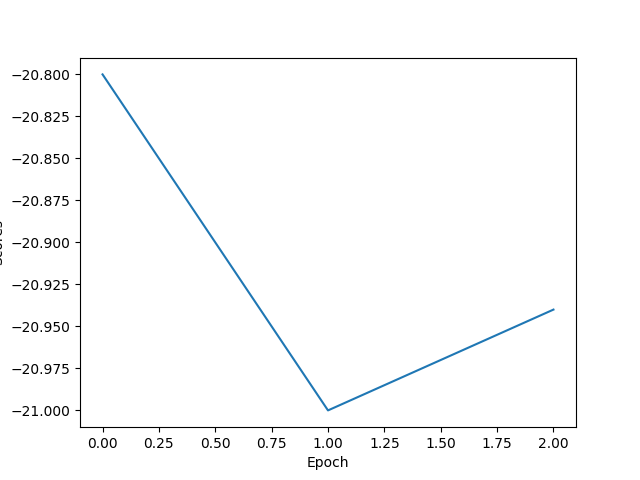
\includegraphics[width=.5\linewidth]{images/q4_linear.png}
  \end{figure}
  The performance of the linear model on the Pong-v5 environment is extremely poor and shows
  no evidence of learning.
  % ### END CODE HERE ###
\end{answer}
% <SCPD_SUBMISSION_TAG>_4a
\clearpage

\LARGE
4.c
\normalsize

% <SCPD_SUBMISSION_TAG>_4c
\begin{answer}
  % ### START CODE HERE ###
  The DQN is obviously improving its performance over time while the linear model doesn't seem
  to improve.

  The DQN has a deep CNN layer that are specifically designed for image data. It gives the DQN
  the understanding of the game state directly from pixels, which is necessary for high-level
  strategic play.

  On the other hand, the linear model treat each pixels as an independent feature and attempts
  to find a simple linear relationship between pixel values and strategy, which is insufficient.
  % ### END CODE HERE ###
\end{answer}
% <SCPD_SUBMISSION_TAG>_4c
\clearpage

\LARGE
4.d
\normalsize

% <SCPD_SUBMISSION_TAG>_4d
\begin{answer}
  % ### START CODE HERE ###
  No, the performance of DQN is improving in the long run but it fluctuate a lot locally.
  It could be the $\epsilon$-greddy exploration where it randomly choose the actions sometimes
  that causes the fluctuation. Also, the deep neural network is a highly non-linear function
  approximation. A small parameter change can lead to significant change in the policy.
  % ### END CODE HERE ###
\end{answer}
% <SCPD_SUBMISSION_TAG>_4d
\clearpage

% <SCPD_SUBMISSION_TAG>_entire_submission

\end{document}
